\documentclass[11pt,a4paper]{article}

\usepackage[utf8]{inputenc}
\usepackage[T1]{fontenc}
\usepackage[ngerman]{babel}
\usepackage{amsmath,amssymb}
\usepackage{graphicx}
\usepackage{booktabs}
\usepackage{geometry}
\usepackage{float}
\usepackage{hyperref}
\usepackage{microtype}

\geometry{margin=2.6cm}
\hypersetup{
  colorlinks=true,
  linkcolor=blue,
  citecolor=blue,
  urlcolor=blue
}

\title{\textbf{Aharonov--Bohm-Phasen, Primzahlvierlinge und arithmetische Von-Klitzing-Stufen}\\
\large Eine numerische Energiedokumentation auf Basis von Riemann-Nullstellen}
\author{Thomas Hoffbauer}
\date{\today}

\begin{document}
\maketitle

\begin{abstract}
Dieser Artikel beschreibt eine numerische Testumgebung, in der ordinäre Riemann-Nullstellen
als diskrete Energieniveaus $\gamma_n$ interpretiert und über gerundete Normschalen
arithmetisch klassifiziert werden. Im Zentrum steht die Aharonov--Bohm-Phasendifferenz
zwischen den Restklassen $1 \bmod 4$ und $3 \bmod 4$. Neben globalen Phasendriften werden
lokale Resonanzen auf Primzahlvierlingen der Form $(p,p+2,p+6,p+8)$ untersucht. Die
resultierenden Vierlings-Plateaus zeigen ein diskretes Stufenmuster, das als arithmetisches
Analogon eines quantisierten Von-Klitzing-Hall-Effekts gelesen werden kann.
\end{abstract}

\section{Einleitung}

Die numerische Konstruktion beginnt mit einem Datensatz von Riemann-Nullstellen
\[
  \rho_n = \frac12 + i\gamma_n,
\]
wobei die Ordinaten $\gamma_n$ als spektrale Energieniveaus verwendet werden. Jede
Nullstelle wird einer ganzzahligen Normschale
\[
  N_n = \operatorname{round}(\gamma_n)
\]
zugeordnet. Die Phase der Nullstelle im Aharonov--Bohm-Sinn wird durch
\[
  \phi_n = \gamma_n \bmod 2\pi
\]
modelliert. Durch die Zerlegung der Normschalen in die Restklassen $1 \bmod 4$ und
$3 \bmod 4$ entsteht eine chirale Phasendifferenz
\[
  \Delta\phi =
  \langle \phi\rangle_{N\equiv 3 \bmod 4}
  -
  \langle \phi\rangle_{N\equiv 1 \bmod 4}.
\]
Diese Größe wird sowohl global über Energieintervalle als auch lokal auf
Primzahlvierlingen ausgewertet.

\section{Numerisches Modell}

Die Implementierung verwendet den Datensatz \texttt{zeros6.npy}. Nach dem Laden der
Nullstellen werden drei arithmetische Projektionen gebildet:
\begin{enumerate}
  \item die gerundeten Normschalen $N_n$,
  \item die Phasen $\phi_n = \gamma_n \bmod 2\pi$,
  \item die Restklassen $N_n \bmod 4$.
\end{enumerate}

Für ein Intervall $I$ von Nullstellen lautet die gemessene Phasendifferenz
\[
  \Delta\phi(I)
  =
  \frac{1}{|I_3|}\sum_{n\in I_3}\phi_n
  -
  \frac{1}{|I_1|}\sum_{n\in I_1}\phi_n,
\]
mit
\[
  I_1=\{n\in I: N_n\equiv 1 \bmod 4\}, \qquad
  I_3=\{n\in I: N_n\equiv 3 \bmod 4\}.
\]

\section{Globale Aharonov--Bohm-Phasen}

Zunächst werden zwei Energieepochen betrachtet: ein tiefer thermischer Bereich und ein
asymptotischer Grenzbereich. Beide Tests messen die Verteilung der Nullstellen auf den
Restklassen $1 \bmod 4$ und $3 \bmod 4$ sowie deren mittlere Phasen. Die Differenz
$\Delta\phi$ fungiert dabei als globale Hintergrundspannung des arithmetischen Systems.

Zusätzlich wird aus der Folge der Nullstellen eine Niveauabstandsverteilung erzeugt. Die
Abstände
\[
  \delta_n = \gamma_{n+1}-\gamma_n
\]
werden als lokale Landau-Niveau-Abstoßung visualisiert.

\IfFileExists{test_env_von_klitzing.png}{
\begin{figure}[H]
  \centering
  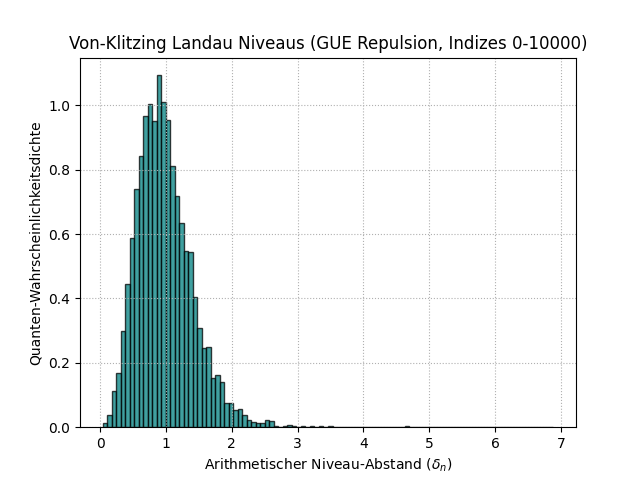
\includegraphics[width=0.82\textwidth]{test_env_von_klitzing.png}
  \caption{Lokale Niveauabstände der Riemann-Nullstellen als Von-Klitzing-Plateau-Analogie.}
  \label{fig:klitzing-local}
\end{figure}
}{}

\section{Thermodynamische Zustandsgleichung}

Zur asymptotischen Analyse wird der Datensatz in $B$ Energieblöcke zerlegt. Für jeden Block
wird der mittlere Energiewert
\[
  \bar{\gamma}_b = \frac{1}{|B_b|}\sum_{\gamma_n\in B_b}\gamma_n
\]
und die zugehörige Phasendifferenz $\Delta\phi_b$ berechnet. Die numerische
Zustandsgleichung wird anschließend durch eine logarithmische Regression modelliert:
\[
  \Delta\phi(\gamma) = a\ln(\gamma)+b.
\]

Diese Gleichung beschreibt den globalen Drift der chiralen Phasendifferenz über die
Energieskala der Nullstellen. Die Steigung $a$ codiert die asymptotische Driftgeschwindigkeit,
während $b$ die extrapolierte Phasenlage fixiert.

\IfFileExists{ab_phase_state_equation.png}{
\begin{figure}[H]
  \centering
  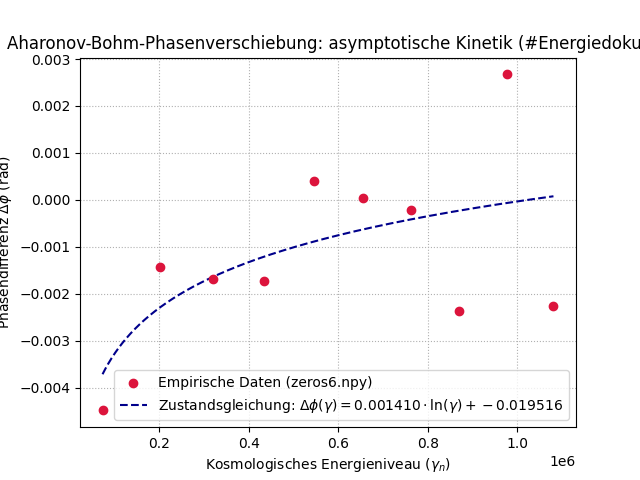
\includegraphics[width=0.82\textwidth]{ab_phase_state_equation.png}
  \caption{Logarithmische Zustandsgleichung der Aharonov--Bohm-Phasendifferenz.}
  \label{fig:state-equation}
\end{figure}
}{}

\section{Primzahlvierlinge als lokale Resonatoren}

Die lokale Resonanzanalyse isoliert Primzahlvierlinge
\[
  Q_p = (p,p+2,p+6,p+8).
\]
Diese Vierlinge besitzen eine natürliche Aufteilung in äußere und innere Schalen. Für
$p\equiv 3 \bmod 4$ liegen die äußeren Komponenten $p$ und $p+8$ ebenfalls in der Klasse
$3 \bmod 4$, während $p+2$ und $p+6$ in der Klasse $1 \bmod 4$ liegen. Daraus entsteht die
lokale Vierlings-Phasendifferenz
\[
  \Delta\phi_Q =
  \left\langle \gamma \bmod 2\pi \right\rangle_{\{p,p+8\}}
  -
  \left\langle \gamma \bmod 2\pi \right\rangle_{\{p+2,p+6\}}.
\]

Ein Vierling gilt als aktiviert, wenn mindestens eine seiner Normschalen von einer
Riemann-Nullstelle getroffen wird. Für den Niedrig/Hoch-Vergleich wird die aktivierte
Vierlingsmenge nach Energie sortiert und in zwei Hälften geteilt. So entsteht ein lokaler
Resonanzvergleich gegen den globalen Hintergrunddrift.

\IfFileExists{quartet_compensation_dynamics.png}{
\begin{figure}[H]
  \centering
  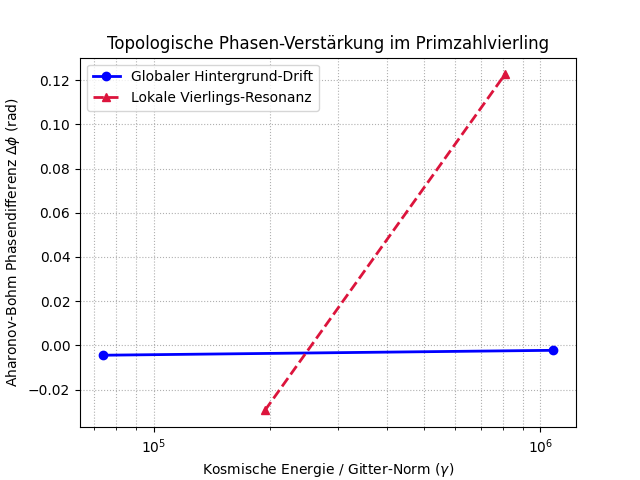
\includegraphics[width=0.82\textwidth]{quartet_compensation_dynamics.png}
  \caption{Vergleich zwischen globalem Hintergrunddrift und lokaler Primzahlvierlings-Resonanz.}
  \label{fig:quartet-compensation}
\end{figure}
}{}

\section{Quantisierte Hall-Stufen}

Im letzten Test werden nur solche Vierlinge betrachtet, bei denen beide chiralen Sektoren
getroffen werden:
\[
  \{p,p+8\}\cap\{N_n\}\neq\varnothing
  \quad\text{und}\quad
  \{p+2,p+6\}\cap\{N_n\}\neq\varnothing.
\]
Für jeden aktiven Vierling wird ein lokales Potential
\[
  V_Q = \Delta\phi_Q
\]
berechnet. Sortiert man diese Werte nach der mittleren Vierlingsenergie
\[
  \gamma_{\mathrm{quad}} = \frac{p+(p+2)+(p+6)+(p+8)}{4}=p+4,
\]
entsteht eine diskrete Sequenz lokaler Plateaus. Die Sprunghöhen
\[
  s_k = V_{Q_{k+1}}-V_{Q_k}
\]
messen die Übergänge zwischen benachbarten Resonanzzentren.

\IfFileExists{von_klitzing_arithmetic_steps.png}{
\begin{figure}[H]
  \centering
  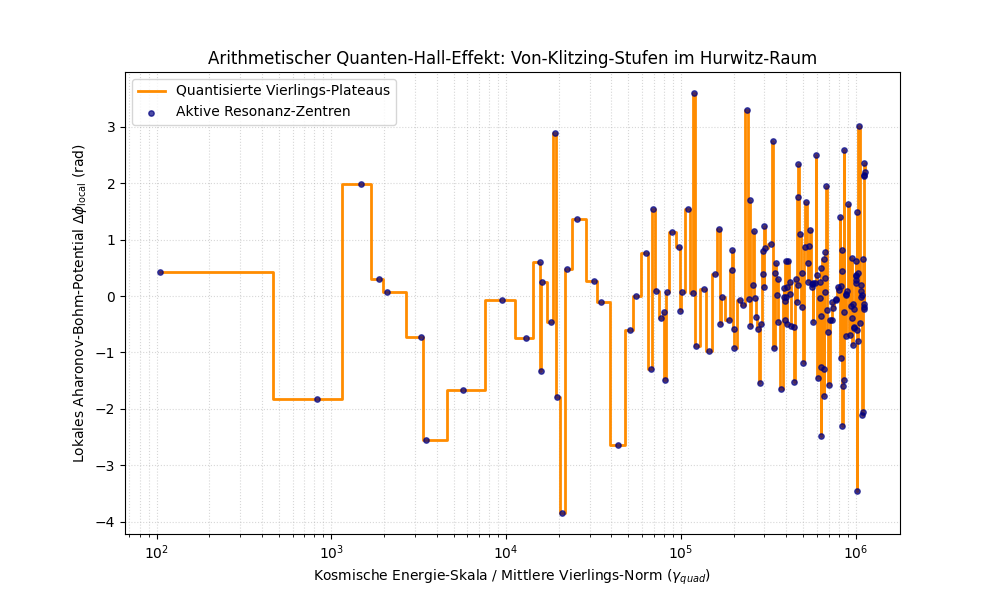
\includegraphics[width=0.82\textwidth]{von_klitzing_arithmetic_steps.png}
  \caption{Diskrete Von-Klitzing-Stufen der lokalen Vierlings-Phasenpotentiale.}
  \label{fig:arithmetic-steps}
\end{figure}
}{}

\section{Zusammenfassung}

Die Tests zeigen eine zweistufige Struktur. Auf globaler Ebene driftet die
Aharonov--Bohm-Phasendifferenz langsam und wird durch eine logarithmische
Zustandsgleichung beschrieben. Auf lokaler Ebene erzeugen Primzahlvierlinge diskrete
Resonanzzentren, deren aktivierte Phasenwerte ein treppenartiges Plateau-Muster bilden.
Damit verbindet das Modell drei arithmetische Ebenen: Riemann-Nullstellen als
Energiespektrum, Restklassen modulo $4$ als chirale Sektoren und Primzahlvierlinge als
lokale topologische Kopplungsstellen.

\section*{Reproduzierbarkeit}

Die numerische Auswertung wird durch das Python-Skript \texttt{Ganteför.py} erzeugt. Der
Hauptlauf lädt \texttt{zeros6.npy}, führt die Tests 1 bis 6 aus und exportiert die
Abbildungen:
\begin{itemize}
  \item \texttt{test\_env\_von\_klitzing.png},
  \item \texttt{ab\_phase\_state\_equation.png},
  \item \texttt{quartet\_compensation\_dynamics.png},
  \item \texttt{von\_klitzing\_arithmetic\_steps.png}.
\end{itemize}

\end{document}
